% Preamble
\documentclass[11pt]{article}

% Packages
\usepackage{a4wide}
\usepackage{graphicx}
\usepackage{url}
\graphicspath{{images/}}
\usepackage[nottoc]{tocbibind}
\usepackage{listings}
\usepackage{caption}
\usepackage{amsmath}

% Author
\author{Van Dam, Thijs\\
\and
Bos, Sander\\
}
\title{\huge The Animal Kingdom}
\date{April 2018}

\setlength{\parindent}{0em}
\setlength{\parskip}{1em}

\DeclareCaptionFormat{cancaption}{#1#2#3\par}
\DeclareCaptionLabelFormat{cancaptionlabel}{#1}
\captionsetup[figure][number]{format=cancaption,labelformat=cancaptionlabel}

% Document

\begin{document}
    \maketitle
    \thispagestyle{empty}
    \newpage
    \newpage
    \setcounter{page}{1}
    \section{Introduction}\label{sec:introduction}
    In this document we discuss the following topics:
    \begin{itemize}
        \item Steering
        \item Path planning
        \item Behaviour
        \item Fuzzy logic
    \end{itemize}
    
    To understand the context of this game, we will first give a short explanation of the game/simulation itself.
    
    \subsection*{About the game}\label{subsec:about}
    Somewhere in Africa, a herd of gazelles is gathering food.
    At the same time a pride of lions is getting quite hungry and thus sees the gazelles as a tasteful meal.
    The gazelles notice the lions are getting closer and closer.
    They start to run.
    It becomes a race of life and death...

    \newpage
    %-----------------------------------------------------------------------------------------
    \tableofcontents
    
    \newpage
    %-----------------------------------------------------------------------------------------
    \section{Steering}\label{sec:steering}

    \newpage
    %-----------------------------------------------------------------------------------------
    \section{Path planning}\label{sec:pathPlanning}
    This section contains all information about the path planning algorithms and structure used in 'The Animal Kingdom'.
First the structure will be discussed, then we will give an illustration of how the graph is rendered and in the last part of this section,
the implementation of the used path-finding algorithms is explained.

\subsection{Structure}\label{subsec:pathstructure}
Buckland describes\cite{pgaie} a well-structured approach to splitting logic for the pathfinding.
This same structure is what we used in our application, although we have made some changes to fit our own needs.
The application contains one instance of a \textit{PathManager} and each (moving) entity contains a \textit{PathPlanner}.
The \textit{PathPlanner} is what is used to request a new search with the specified algorithm (A* or Dijkstra).
When a request is done, the \textit{PathPlanner} registers itself in the \textit{PathManager}.
Using a \textit{PathManager} makes it possible to manage and control all search requests from one place.
This is especially useful when you want to implement time-slicing or other logic that restricts the amount of search cycles per update.
The latter case is what we use it for.
\textit{PathManager} contains a function \textit{UpdateSearches()} which lets each \textit{PathPlanner} do one or more cycle depending on the maximum cycles set while instantiating the \textit{PathManager}.
What a cycle does, will be discussed in section \ref{subsec:pathalgorithms}.\par
The class diagram below (fig.\ref{fig:pathPlanClassDiagram}) shows the structure of the pathfinding logic including the \textit{PathManager} and \textit{PathPlanner}.

\begin{figure}[h!]
    \begin{center}
        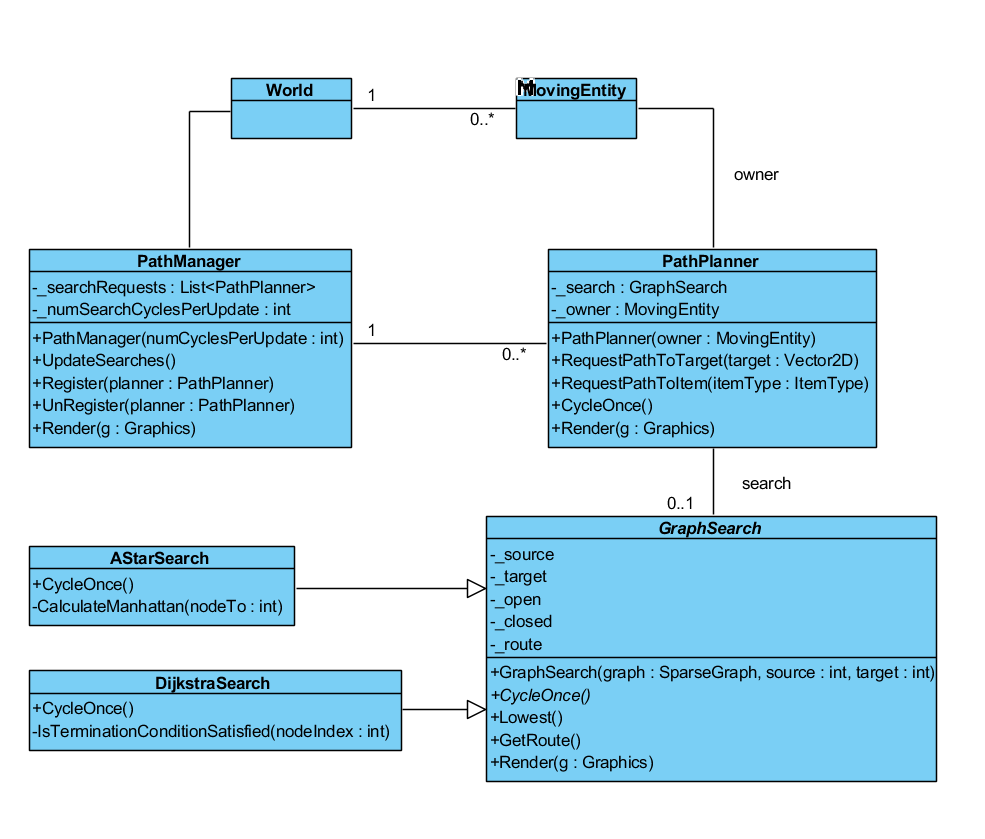
\includegraphics[width=26em]{PathFinding.png}
    \end{center}
    \caption{Path planning class diagram}
    \label{fig:pathPlanClassDiagram}
\end{figure}

\subsection{Creating a graph}\label{subsec:pathgraphcreation}
The graph in the game world is created using a floodfill.
A single point is given as its starting position and from that point edges and nodes are added in every direction.
If the placing of an edge or node is obstructed by an obstacle, it will not be created and the floodfill will continue
in the other directions.
This results in a graph that fills the complete game world.
The graph itself is not saved as a file, it is possible to do this, but because of the small area of the field,
generating a graph at the start of the application does not affect performance and loading time.
The picture below (fig.\ref{fig:pathPlanFloodfill}) demonstrates the result of using floodfill.

\begin{figure}[h!]
    \begin{center}
        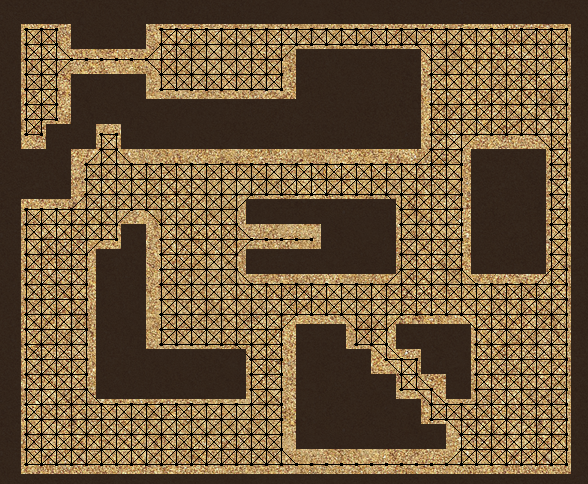
\includegraphics[width=28em]{Floodfill.png}
    \end{center}
    \caption{The result of using floodfill}
    \label{fig:pathPlanFloodfill}
\end{figure}

\subsection{Algorithms}\label{subsec:pathalgorithms}
As mentioned previously, we have implemented two path-finding algorithms in the application.
Dijkstra and A*. Each of the algorithms is implemented in a separate class extending the \textit{GraphSearch} class.
Both implementations will be discussed below.

\subsubsection{Dijkstra}\label{sec:pathDijkstra}
The first algorithm we implemented, is Dijkstra as it is also the base of the A* algorithm.
Although the algorithm was already familiar to us, implementing it was a bit more difficult than we expected.
It was not a lot of work, but it did require some thinking.
In Programming Game AI by Example, Buckland describes a version of the algorithm that looked more complex than necessary.
Luckily we found a pseudo code\cite{aapc} of A*, which by removing the heuristics, was a much better understandable version of the algorithm.\par
A first version of the algorithm was without the \textit{PathManager} and/or \textit{PathPlanner} and did not contain the \textit{CycleOnce()}.
Instead, we had a single function \textit{Search()} which did the whole search at once.
The function \textit{IsTerminationConditionSatisfied()} was added to check if an item of the specified \textit{ItemType} was found.
If a matching item was found, the algorithm was stopped and the route was returned.
The resulting route was eventually drawn on the screen by adding a \textit{Render()} function.

\subsubsection{A*}\label{sec:pathAstar}
As A* is basically Dijkstra with heuristics, it was easy to convert our existing Dijkstra algorithm to A*.
Just as with the Dijkstra algorithm, we first created a single \textit{Search()} which did the whole search at once.
The heuristic used for our implementation is Manhattan, which we calculated in \textit{CalculateManhattan()}.
The distance between all nodes is the same in the graph and each edge has a cost of 1.
Calculating the Manhattan distance was very easy as we could just calculate the distance between the current node and target location
and devide it by the length of one edge to get the estimated distance (fig.\ref{fig:pathPlanCalcManhattan}).

\begin{figure}[h!]
    \[ $$Dist_M = \dfrac{|targetLocation.X - currentLocation.X| + |targetLocation.Y - currentLocation.Y|}{15}\]
    \caption{Calculating the Manhattan distance}
    \label{fig:pathPlanCalcManhattan}
\end{figure}

\subsection{Performance}\label{subsec:pathperformance}
Because of the implementation of the \textit{PathManager} and \textit{PathPlanner} resources will be shared equally between all moving entities.
There is also a predifined maximum amount of calculation cycles per update, which prefents the game from slowing down.
At first we struggled with this, as it seemed to take much longer to find a path than previoulsy with just the single \textit{Search()} function.
After a bit of tweaking (changing the maximum amount of cycles per update) and removing a lot of \lstinline[columns=fixed]{Console.WriteLine(...)}
lines used for debugging which were clearly slowing down the calculations as they were limited by the speed of the console.\par
However, performance can still be improved.
Storing precalculated costs, or some shortest paths could dramatically improve the performance when the amount of agents increases.

    \newpage
    %-----------------------------------------------------------------------------------------
    \section{Behaviours (Goals)}\label{sec:behaviour}
    Behaviour of all entities within the game are discussed in this section.

\subsection{Structure}\label{subsec:behaviourStructure}
We have chosen to use goal-driven behaviour in our game.
Three main classes make up most of the structure, they are: \textit{Goal}, \textit{CompositeGoal} and \textit{AtomicGoal}.
As seen in the naming, a composite design pattern has been used to enable the grouping of goals while keeping the same functionalities.
This means that an \textit{AtomicGoal} can be used in the same way as a \textit{CompositeGoal} with the exception of \textit{AddSubGoal()},
which is only implemented in the composite.
This structure is used to create all strategy-level goals.

The class diagram below shows the structure (fig.\ref{fig:behaviourClassDiagram}).

\begin{figure}[h!]
    \begin{center}
        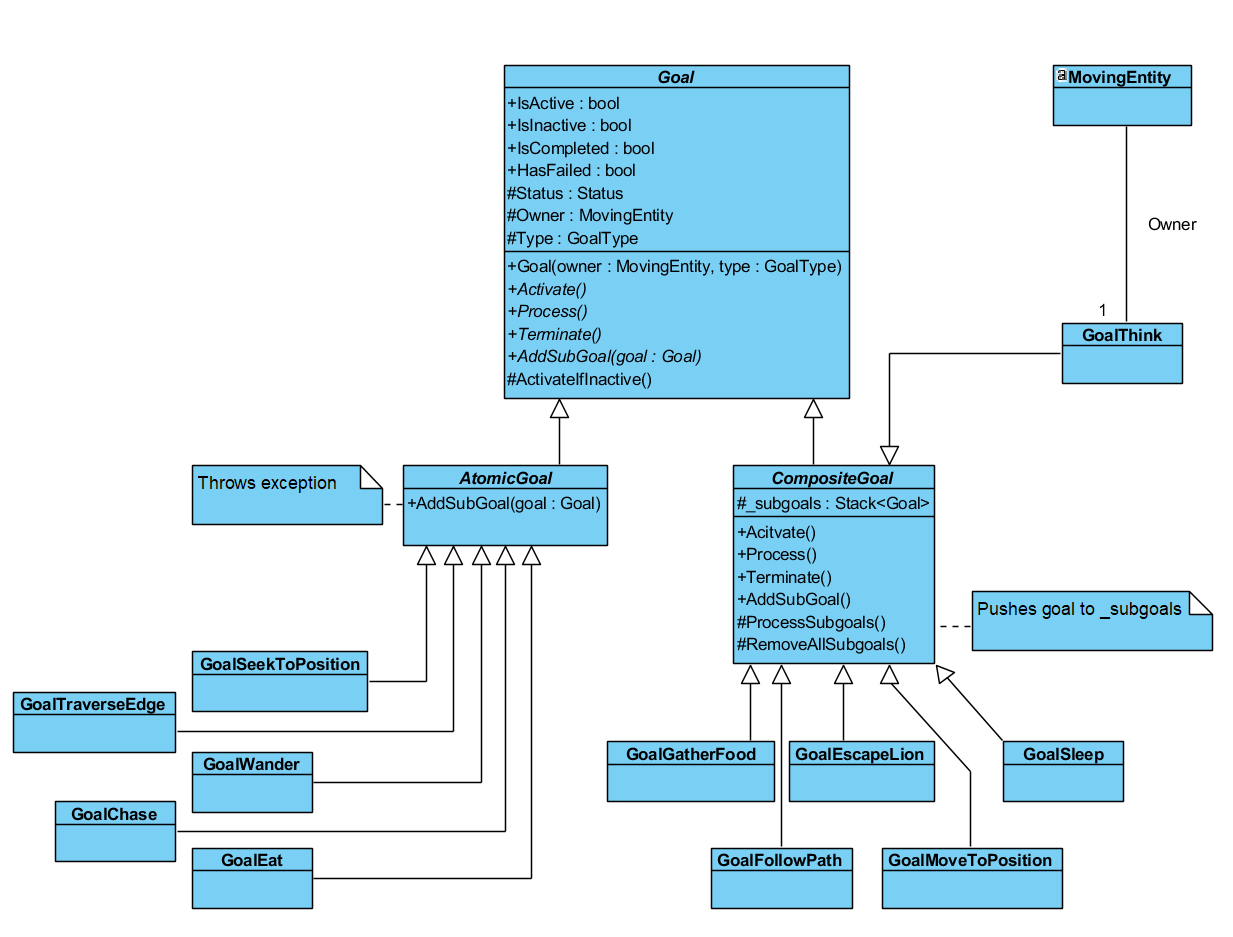
\includegraphics[width=40em]{Goals.png}
    \end{center}
    \caption{Goals class diagram}
    \label{fig:behaviourClassDiagram}
\end{figure}


\subsection{Goals}\label{subsec:behaviourGoals}
To give each entity a specific behaviour, we have created a couple of (composite) goals with some underlying atomic goals.
These goals wil be discussed below.

\subsubsection{Gather Food}\label{sec:behaviourFood}
Both the gazelles and the lions will have to gather food if they want to survive.
For gazelles it will mean that they have to find (\textit{GoalMoveToPosition}) grass or water and start eating.
Lions do not like grass, so they will have to chase (\textit{GoalChase}) a gazelle and eat it.
The gazelle will then try to escape (\textit{GoalEscapeLion}) which we will discuss in the next part.
If a lion caught a gazelle, the lion will eat (\textit{GoalEat}) the poor animal.

This is the most complex behaviour.
The \textit{GoalMoveToPosition} has as its first subgoal \textit{GoalSeekToPosition}.
This will continue until the path has been found and then \textit{GoalFollowPath} will be added with the found path.
While there is a path to follow, the \textit{GoalTraverseEdge} will be added, each time with a next node as position to travel to.
This enables the \textit{SeekBehaviour} to the given point.
If it is the last node, the \textit{GoalTraverseEdge} will start the \textit{ArriveBehaviour} to the final destination.

\subsubsection{Escape From Lion}\label{sec:behaviourEscape}
A gazelle does not want to be eaten by a lion, so it will try to escape a lion once it is within a certain range.
The \textit{FleeBehaviour} will be enabled for the gazelle, but its energy will drain.
%ToDo: Do we want flee or not, what should we do with this goal?

\subsubsection{Sleep}\label{sec:behaviourSleep}
Lions are actually lazy animals.
Once they had a nice meal, they want to sleep.
Gazelles will be very happy once that happens and they can relax for a while.
They will probably start grazing again as that is what they do most of the time.
If a lion sleeps, it won't do anything for a while, until he is fully back to strength.

This is a pretty simple goal, but very important for the lions.
It will temporarily disable all steering behaviour for the lion entity.


    
    \newpage
    %-----------------------------------------------------------------------------------------
    \section{Fuzzy logic}\label{sec:fuzzyLogic}

    \newpage
    %-----------------------------------------------------------------------------------------
    \section{Conclusion}\label{sec:conclusion}
    \subsection[Reflection on the end result]{Reflecion}\label{subsec:reflection}
Looking back at this project I think we did a pretty good job.
Since it was a school exercise we wanted to get it done really fast, and sometimes the development lacked of some testing.
Yet, we tested it good enough to pass working parts of the program to eachother.
So, actually, the not testing wasn't really in our way!
It mainly left some insecurities and we had to hope for the code to work.

Then we wanted to implement everything on the best, neatest possible way and I think that was in our way sometimes.
This way we lost a lot of time thinking things through that actually were finished already.

In the beginning we did a lot of paired programming and I think this cost a lot of time as well.
Mostly since you simply don't have the producing code of two programmers, but of only one.

Looking at these point, you may notice that there was a severe lack of time.
We actually spent a lot of hours on this project, but it was really hard work to get it done in time.

\subsection[Improvements of our project]{Improvements}\label{subsec:improvements}
There are some big improvements that can be done to our game.
This is mainly aimed at the looks of the game, the use of sprites and the behaviours of the animals.

Currently we only used images and not really sprites to represent our entities, this could be a lot better if we just used sprites!
Once again, this was mainly because the lack of time we had.

Then the behaviour of the animals.
With this I mean that we had a limit to how many fuzzy modules / sets we could implement.
The currently implemented fuzzy logic only handles if a gazelle wants to eat or to run from a lion.
The lion can't even decide if it goes after a gazelle yet!
That is a big bummer, because it would be a lot more interactive if this did work.

We also didn't take into account that entities wont flee from another entity if there is an obstacle inbetween.
Right now, we just run from the other entity no matter what.
This would be a pretty easy, but quite essential modification.
Mostly since the gazelle would actually hide behind something and this would look pretty realistic.

The last big improvement I can think of, is some better implementation of the FuzzyLogic into the GoalManager.
Right now we just created a static FuzzyManager to get all configurations for the FuzzyLogic.
We could've implemented this inside the GoalManager much more beautiful (for \textbf{instance} (hehe..) a non-static class).

    \newpage
    %-----------------------------------------------------------------------------------------

    \addcontentsline{toc}{chapter}{References}
    \begin{thebibliography}{9}
        \bibitem{pgaie}
        Mat Buckland (2004).
        \textit{Programming Game AI by Example}.
        Wordware, 2004

        \bibitem{aapc}
        Lluis Alseda.
        \textit{A* Algorithm pseudocode}
        \\\textit{\url{http://mat.uab.cat/~alseda/MasterOpt/AStar-Algorithm.pdf}}
        \\\textit{Accessed: 2018-04-01}
    \end{thebibliography}
\end{document}